\chapter{Stochastic Differential Equations COMING SOON}
\label{ch-stochastic-diff-eqns}


Stochastic Differential Equation (SDE)
First order differential equation with noise

Ref.\cite{sde-applied-book}

\section{Notation}

$[a, b]=\{ x\in \RR: a\leq x \leq b\}$

Suppose $i, j\in \{0, 1, \ldots, N-1\}$

$[i \upto j] = [i, i+1, \ldots, j]$

$[i:j] = [i, i+1, \ldots, j-1]$


$[n]=[0:n]=\{0, 1, 2, \ldots, n-1\}$


Suppose $t_0=0<t_1<t_2<\ldots < t_{N-1}$



$t_{[i\upto j]} = [t_i, t_{i+1}, \ldots, t_j]$


\beq
\lim_{N\rarrow \infty}t_{[i\upto j]} =
[t_i, t_j]
\eeq



Path

$\rvx([t,s])=\{  \rvx(\tau): \tau\in[t,s]\}$


$\rvx(t_{[j\upto k]}) =\{  x(\tau): \tau\in\{t_j, t_{j+1}, \ldots, t_k\}\}$

$\rvx_{[j\upto k]} =\{ \rvx_j, \rvx_{j+1},
\ldots,\rvx_k\}$


Measure theorists speak of a family of sigma algebras wherein the elements of the family increase with $t$. They call this a {\bf filtration}. A path $x([t, s])$ is equivalent to a filtration,
so we won't speak of filtrations here.



$dx^n = dx_0 dx_1 \ldots dx_{n-1}$

\beq 
\av{\rva} = E[\rva]
\eeq

\beq
\Delta \rva = \rva - \av{\rva}
\eeq

\beq
Cov(\rva, \rvb) =\av{\rva, \rvb}=
\av{\Delta\rva \Delta\rvb}
\eeq

\beq
\Delta_{t_0}^{t_1}a = a(t_1) - a(t_0)
\eeq



random process $\rvx(t)$ for $t\geq 0$

$t_0=0 < t_1 < t_2 <\ldots< t_{N-1}$

sequence of random variables $\rvx(t_0),
 \rvx(t_1), \rvx(t_2), \ldots \rvx(t_{N-1})$
 
Will often define $\rvx(t_i) =\rvx_i$.

Will use lower case Latin indices for time
and Greek letters for $\rvx\in\RR^n$ components.
Hence $\rvx_{\mu, i}=\rvx_\mu(t_i)$



 
 \section{White Noise and Brownian Motion}
 
 \begin{figure}[h!]
 \centering
 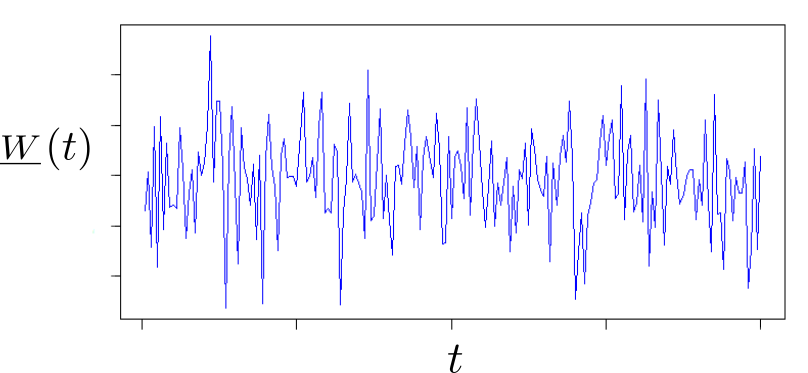
\includegraphics[width=4in]
 {stochastic-diff-eqns/white-noise-labeled}
 \caption{One dimensional white noise $\rvW(t)$}
 \label{fig-white-noise-t}
 \end{figure}
 
 \begin{figure}[h!]
  \centering
  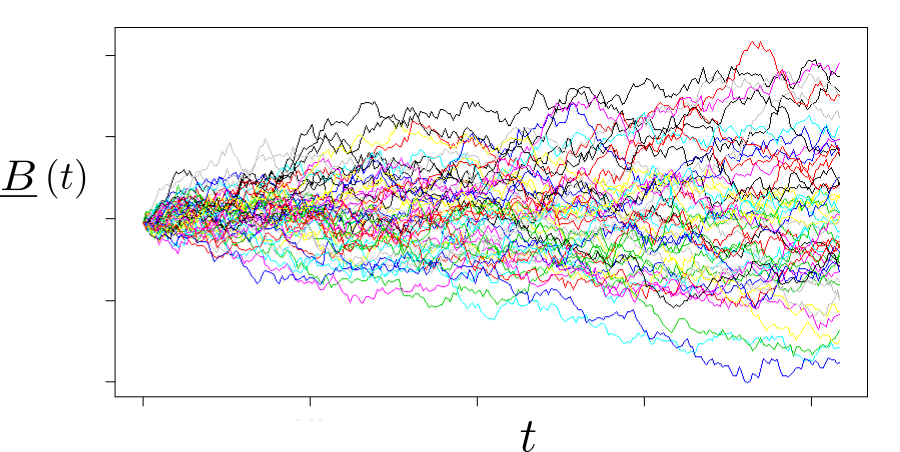
\includegraphics[width=4in]
  {stochastic-diff-eqns/brownian-motion-labeled}
  \caption{One dimensional Brownian motion $\rvB(t)$}
  \label{fig-brownian-motion-t}
  \end{figure}
  
 

White noise $\rvW(t)
\in\RR^n$ for $t\geq 0$

\begin{enumerate}
\item
\beq
\rvW(t) \sim \caln(\mu=0, Cov=Q)
\eeq

\item
$\rvW(t)$ and $\rvW(s)$ independent for
$t\neq s$

\item

\beq E[\rvW(t)]=0
\eeq

\item
\beq
C_\rvW(t, s) = \av{\rvW(t), \rvW^T(s)} = Q\delta(t-s)
\eeq



\end{enumerate}
Brownian motion (a.k.a. as a Wiener process) $\rvB\in\RR^n$
for $t\geq 0$

\begin{enumerate}

\item

\beq 
\rvB(0)=0\footnote{For $\rvB(0)=\beta_0\neq 0$, replace
$\rvB$ by $\rvB-\beta_0$}
\eeq

\item

\beq
\frac{
\Delta_{t_k}^{t_{k+1}}\rvB
}{\Delta_{t_k}^{t_{k+1}}t}
\sim \caln(\mu=0, Cov=Q)
\eeq

\beq
\rvW(t_k)\sim  \caln(\mu=0, Cov=Q)
\eeq

\beq
\frac
{d \rvB}{dt} = \rvW
\eeq


\item

\beq
E[(\Delta^{t}_{s}\rvB)^2] = n|t-s|
\eeq
where $\rvB(t)\in\RR^n$


\item
If $[r, s]\cap [r', s']=\emptyset$ then

\beq
E[(\Delta^{s}_{r}\rvB) (\Delta^{s'}_{r'}\rvB)]=0
\eeq


\beqa
E[\Delta_1^4\rvB \Delta_3^6\rvB]
&=&
E[(\Delta_1^3\rvB + \Delta_3^4\rvB)
(\Delta_3^4\rvB + \Delta_4^6\rvB)
]
\\
&=&
E[(\Delta_3^4\rvB)^2]
\\
&=& n |4-3|
\eeqa

In general

\beq
E[(\Delta^{s}_{r}\rvB) (\Delta^{s'}_{r'}\rvB)]=n {\rm len}([r, s]\cap [r', s'])
\eeq

\end{enumerate}


\section{SDE bnet}

special nodes

We discussed marginalizer nodes in Chapter
\ref{ch-marginalizer}.

\begin{itemize}

\item {\bf diff ad diff0} 

$$\xymatrix{
\rva\ar[dr]
&&\rvb\ar[dl]
\\
&
\rvx
}
$$

\beq  \color{blue}
P(x|a, b) =\indi (x =a-b)
\eeq

\beq  \color{blue}
x =a-b
\eeq
 diff0 node is the diff node with $x=0$
 


\item {\bf accumulator}

$$
\xymatrix{
\rvx_3 \ar[d]
&\rvx_2\ar[d]
&\rvx_1\ar[d]
&\rvx_0\ar[d]
\\
\rvs_3 
&\rvs_2\ar[l]
 &\rvs_1\ar[l]
  &\rvs_0\ar[l]
}$$



\beq
\color{blue}
\begin{array}{lll}
\rvs_3 &=& \rvx_3 + \rvs_2
\\
\rvs_2 &=& \rvx_2 + \rvs_1
\\
\rvs_1 &=& \rvx_1 + \rvs_0
\\
\rvs_0&=& x_0
\end{array}
\eeq

\item {\bf incrementer}

$$
\xymatrix{
\rvB_3\ar[dr] 
&& \rvB_2\ar[dl]\ar[dr]
&& \rvB_1\ar[dl]\ar[dr]
&& \rvB_0\ar[dl]
\\
&\Delta^3_2\rvB 
&&\Delta^2_1 \rvB 
&&\Delta^1_0 \rvB
&
}$$

\beq\color{blue}
\begin{array}{lll}
\Delta_2^3\rvB &=& \rvB_3 - \rvB_2
\\
\Delta_1^2\rvB &=& \rvB_2 - \rvB_1
\\
\Delta_0^1\rvB &=& \rvB_1 - \rvB_0
\end{array}
\eeq

\item {\bf de-incrementer}
$$
\xymatrix{
&\Delta^3_2\rvx_2 \ar[dl] 
&&\Delta^2_1 \rvx \ar[dlll]\ar[dl]
&&\Delta \rvx^1_0 \ar[dlllll]\ar[dlll]\ar[dl]
&
\\
\rvx_3 
&& \rvx_2 
&& \rvx_1
&& \rvx_0
\ar@/^1pc/[ll]
\ar@/^1pc/[llll]
\ar@/^1pc/[llllll]
}
$$
\beq
\color{blue}
\begin{array}{lll}
\rvx_3 &=& \Delta_2^3\rvx + \Delta_1^2\rvx
+ \Delta^1_0\rvx + x_0
\\
\rvx_2 &=& \Delta_1^2\rvx
+ \Delta^1_0\rvx + x_0
\\
\rvx_1 &=&
\Delta^1_0\rvx + x_0
\\
\rvx_0&=&x_0
\end{array}
\eeq
\end{itemize}


$\rvx, \rvB\in \RR$
\beq
d\rvx= f(\rvx, t)dt + L(\rvx, t)d\rvB(t)
\eeq

\begin{figure}
$$
\xymatrix{
\rvB_3\ar@[red][dr] 
&& \rvB_2\ar@[red][dl]\ar@[red][dr]
&& \rvB_1\ar@[red][dl]\ar@[red][dr]
&& \rvB_0\ar@[red][dl]
\\
&\Delta^3_2\rvB \ar[d]
&&\Delta^2_1 \rvB \ar[d]
&&\Delta^1_0 \rvB \ar[d]
&
\\
&\Delta^3_2\rvx \ar@[green][dl] 
&&\Delta^2_1 \rvx \ar@[green][dlll]\ar@[green][dl]
&&\Delta^1_0\rvx \ar@[green][dlllll]\ar@[green][dlll]\ar@[green][dl]
&
\\
\rvx_3 
&& \rvx_2 \ar[lu] 
&& \rvx_1 \ar[lu]
&& \rvx_0\ar[lu]
\ar@[green]@[green]@/^1pc/[ll]
\ar@[green]@/^1pc/[llll]
\ar@[green]@/^1pc/[llllll]
}
$$
\caption{Bnet for general SDE with $N=4$ number of times. Note that this bnet
contains within it first an incrementer bnet
(in red) for the $\rvB_i$
then a de-incrementer bnet (in green)
for the $\rvx_i$.}
\label{fig-sde-3-nodes}
\end{figure}


\beq
\color{blue}
\Delta_{2}^{3}\rvB = 
\rvB_3 -\rvB_2
\eeq

\beq
\color{blue}
\Delta_{2}^{3}\rvx = 
f(x_3, t)\Delta_2^3 t +
L(x_3, t)\Delta_{2}^{3}\rvB
\eeq

\beq\color{blue}
\rvx_3 = \Delta_{2}^{3}\rvx
+\Delta_{1}^{2}\rvx
+\Delta_{0}^{1}\rvx
+x_0
\eeq

\section{Simple properties of SDE}

\subsection {Transition Matrices}
\subsection{Markov chain}
\subsection{Chapman-Kolgomorov Equation}
Let $x(t_k) = x_k$

\beq
P(x_3|x_1) =\int dx^n_2\; P(x_3|x_2)P(x_2|x_1)
\eeq

\beqa
P(x_3, x_2|x_1) &=&
P(x_3|x_2, x_1)P(x_2|x_1)
\\
&=&
P(x_3|x_2)P(x_2|x_1)
\eeqa



\subsection{Martingale}

For $t, t_i < T$

\beq
E[\;|\rvy(t_i)|\;] < \infty \quad
(E[\;|\rvy(t)|\;] < \infty) 
\eeq


\beq
E\left[\rvy(t)|x(t_{[i\upto j]})\right]= y(t_j)
\quad (E\left[\rvy(t)|x([0,s])\right]= y(s))
\eeq


Brownian motion is a martingale.
\beq
E[\rvB(t)| B(t_{[i\upto j]}] = B(t_j)
\eeq


It\^{o} integrals $\int L(\rvx(t), t)d\rvB(t)$
are martingales too, but Stratonovich
aren't. 



\section{It\^{o} Integral}

Consider 1 dimensional case $\rvx, \rvW\in \RR$.
\beq
\frac{d\rvx}{dt}= f(\rvx, t) + L(\rvx, t)\rvW(t)
\eeq

\beq
\rvx(t) - \rvx(0) =
\int_{0}^{t}dt\; f(\rvx(t), t) + J
\eeq

\beq
J = \int_{0}^t dt\;
L(\rvx(t), t)\rvW(t)
\eeq

$t_0=0 < t_1 <\ldots <t_{N-1}$, $t_k^*\in [t_k, t_{k+1})$

\beq 
J = \lim_{N\rarrow \infty} J_N
\eeq


\beq 
J_N = 
\sum_k L(\rvx(t_k^*), t_k^*)\Delta_{t_k}^{t_{k+1}}\rvB
\eeq


Suppose $L=\rvx=\rvB$

\beq
J_N=\sum_k \rvB(t_k^*) \Delta_{t_k}^{t_{k+1}}\rvB
\eeq

\begin{enumerate}

\item $t_k^* = t_k$, Ito integral\footnote{More precisely,
It\^{o}}


\beqa
E[J_N] &=&\sum_k E[\rvB(t_k)\Delta_{t_k}^{t_{k+1}}\rvB] 
\\
&=& \sum_k
E[(\Delta_{0}^{t_k}\rvB)\Delta_{t_k}^{t_{k+1}}\rvB] 
\\
&=&0
\eeqa

\beqa
J_N &=& 
\sum_k \rvB(t_k)\Delta_{t_k}^{t_{k+1}}\rvB
\\
&=&
\frac{1}{2}\sum_k\left[
-[\Delta_{t_k}^{t_{k+1}}\rvB]^2
+ \Delta_{t_k}^{t_{k+1}}(\rvB^2)\right]
\eeqa

\beqa
J &=& \lim_{N\rarrow \infty} J_N
\\
&=&
\frac{1}{2}
(-t+\rvB^2(t))
\eeqa
$E[J] = \frac{1}{2}(-t+t)=0$



\item $t_k^* = t_{k+1}$ 
\beqa
E[J_N] &=&
\sum_k E[\rvB(t_{k+1})\Delta_{t_k}^{t_{k+1}}\rvB] 
\\
&=&
\sum_k
E[(\Delta_{0}^{t_{k+1}}\rvB)\Delta_{t_k}^{t_{k+1}}\rvB] 
\\
&=&
\sum_k
E[(\Delta_{t_k}^{t_{k+1}}\rvB)^2]
\\
&=&t
\eeqa



\beq
d[\rvB^2(t)]=
2\rvB(t)d\rvB(t)
+t
\eeq


\beq
[d\rvB(t)]^2 = dt
\eeq



\item $t_k^* = \frac{t_k + t_{k+1}}{2}$
Stratonovich integral

\end{enumerate}

For $\rvB\in\RR^n$,

\beq
\boxed{
d[\rvB_\alpha(t)\rvB_\beta(t)]=\delta(\alpha, \beta)
\left[
2\rvB_\alpha(t)d\rvB_\alpha(t)
+nt\right]}
\eeq

\beq
\boxed{
d[\rvB_\alpha(t)]d[\rvB_\beta(t)]
=Q_{\alpha, \beta}dt}
\eeq



\section{Some explicitly solvable examples}
Let $\mu, \nu, \alpha, \beta\in [n]$
\beq
d\rvx_\mu= f(\rvx, t)dt + L(\rvx, t)d\rvB_\mu(t)
\eeq


\beq
\pder{P}{t}= 
\pder{}{x_\mu}\left[-
Pf_\mu + \frac{1}{2}
\pder{}{ x_\nu}(PL_{\mu,\alpha}Q_{\alpha,\beta}L^T_{\beta,\nu})\right]
\eeq

\begin{itemize}

\item
{\bf Brownian motion} ($f_\mu=0$, $(LQL^T)_{\mu,\nu}=2D\delta(\mu, \nu)$)

\beq
dx_\mu =d\rvB_\mu
\eeq


\item {\bf Overdamped Langevin Equation}
($f_\mu=-\frac{1}{2}\pder{U}{x_\mu}$, $(LQL^T)_{\mu,\nu}=2D\delta(\mu, \nu)$)

\beq
dx_\mu = -\;\frac{1}{2}\pder{U}{x_\mu}dt + d\rvB_\mu
\eeq

\item {\bf Ornstein–Uhlenbeck process (a.k.a. Langevin equation)} ($f_\mu=-\lam x_\mu$, $(LQL^T)_{\mu,\nu}=2D\delta(\mu, \nu)$)

This is the same as the Langevin equation, if identify $\rvx$ with
the velocity of the 
particle and $\lam$ with the drag coefficient.


\beq
d\rvx = -\lam \rvx dt + d\rvB
\eeq

\item 
{\bf 1-dim ($n=1$) Black-Sholes} ($f=a x$, $(LQL^T)=(b\rvx)^2 q$)

\beq
d\rvx = a \rvx dt + b \rvx d\rvB
\eeq

\item {\bf 1-dim ($n=1$) General SDE}
($f=a x + c$, $(LQL^T)=(b\rvx + d)^2 q$)


\beq
d\rvx = [a(t)\rvx +c(t)]dt + [b(t)\rvx+ d(t)]d\rvB
\eeq


\beq
x(t) =\Psi(t, t_0)
\left(
x(t_0)
+
\int_{t_0}^{t}ds\;\Psi^{-1}(s, t_0)[c(s)-b(s)]
+
\int_{t_0}^{t}
\Psi^{-1}(s, t_0)d(s)d\rvW(s)
\right)
\eeq

\beq
\Psi(t, t_0)=
\exp\left(
\int_{t_0}^t ds\; \left[a(s)-\frac{1}{2}b^2(s)\right]
+
\int_{t_0}^t b(s) d\rvW(s)
\right)
\eeq



\end{itemize}


\section{Fockker-Planck Equation}


Consider $n$ dimensional case $\rvx, \rvW\in \RR^n$. Let $\mu, \nu,\alpha, \beta\in [n]$.
\beq
d\rvx_\mu= f(\rvx, t)dt + L(\rvx, t)d\rvB_\mu(t)
\eeq

\begin{claim}
\beq
d\phi=
\left[\pder{\phi}{t} +
\pder{\phi}{x_\mu} f_\mu +
\frac{\partial^2\phi}{\partial x_\mu\partial x_\nu}L_{\mu,\alpha}Q_{\alpha,\beta}L^T_{\beta,\nu}\right]dt
+
\pder{\phi}{x_\mu}L_{\mu,\nu}d\rvB_\nu
\eeq
\end{claim}
\proof






\beq
d\phi =
\pder{\phi}{t}dt
+
\sum_\mu \pder{\phi}{x_\mu} d\rvx_\mu
+\frac{1}{2}
\sum_\mu \sum_\nu \frac{\partial^2\phi}{\partial x_\mu\partial x_\nu}d\rvx_\mu d\rvx_\nu
\eeq


\beq
\pder{\phi}{x_\mu} d\rvx_\mu
=
\pder{\phi}{x_\mu} 
\left[
f_\mu dt + L_{\mu, \nu}d\rvB_\nu
\right]
\eeq

\beqa
\frac{\partial^2\phi}{\partial x_\mu\partial x_\nu}d\rvx_\mu d\rvx_\nu
&=&\frac{\partial^2\phi}{\partial x_\mu\partial x_\nu}
\left[
f_\mu dt + L_{\mu, \alpha}d\rvB_\alpha
\right]
\left[
f_\nu dt + L_{\nu, \beta}d\rvB_\beta
\right]
\\
&=&
\frac{\partial^2\phi}{\partial x_\mu\partial x_\nu}
L_{\mu, \alpha}  L_{\nu, \beta} d\rvB_\alpha d\rvB_\beta
\\
&=&
\frac{\partial^2\phi}{\partial x_\mu\partial x_\nu}
L_{\mu, \alpha}  L_{\nu, \beta} Q_{\alpha,\beta} dt
\eeqa

\beqa
d\phi &=&
\pder{\phi}{t}dt
+
\pder{\phi}{x_\mu} [f_\mu dt + L_{\mu,\nu}d\rvB_\nu]
+ \frac{1}{2}
\frac{\partial^2\phi}{\partial x_\mu\partial x_\nu}L_{\mu,\alpha}Q_{\alpha,\beta}L^T_{\beta,\nu}dt
\\
&=&
\left[\pder{\phi}{t} +
\pder{\phi}{x_\mu} f_\mu + \frac{1}{2}
\frac{\partial^2\phi}{\partial x_\mu\partial x_\nu}L_{\mu,\alpha}Q_{\alpha,\beta}L^T_{\beta,\nu}\right]dt
+
\pder{\phi}{x_\mu}L_{\mu,\nu}d\rvB_\nu
\eeqa

\qed

$\rvx(0)=x_0$

Example,  $n=1$, $\rvx=\rvB$, 
$\phi = \rvB^K$

$L=Q=1$, $f=0$

\beq
d(\rvB^K) = K(K-1) \rvB^{K-2}dt
+ K\rvB^{K-1}d\rvB
\eeq

$P(x, t)$
Fokker-Planck equation (FP) (a.k.a. Fokker-Planck-Kolgomrov equation)
\begin{claim} FP for probability of $P(x, t)$
	of single event $(x,t)$
Let

\beq
\calh_\rvx \bullet=
\pder{}{x_\mu}\left[-
(\bullet f_\mu) + \frac{1}{2}
\pder{}{ x_\nu}(\bullet L_{\mu,\alpha}Q_{\alpha,\beta}L^T_{\beta,\nu})\right]
\eeq
Then $P(x,t)$ satisfies

\beq
\pder{P}{t}= \calh_\rvx P
\eeq
which is solved formally by

\beq
P(t)=e^{(t-t_0)\calh_\rvx}P(t_0)
\eeq


\end{claim}
\proof

\beq
\int dx^n\; P(x, t)\left[ \pder{\phi}{x_\mu}L_{\mu,\nu}d\rvB_\nu
\right]
=0
\eeq

Integration by parts

\beq
udv = d(uv)-(du)v 
\eeq

\beq
\int_{-\infty}^{+\infty}udv=
\underbrace{uv|_{-\infty}^{+\infty}}_{0}
\quad
-
\int_{-\infty}^{+\infty}(du)v 
\eeq



\beq
\int dt dx^n\; P(x, t)\frac{d\phi}{dt}=
\int dt dx^n\; P(x, t)
\left[\pder{\phi}{t} +
\pder{\phi}{x_\mu} f_\mu + \frac{1}{2}
\frac{\partial^2\phi}{\partial x_\mu\partial x_\nu}L_{\mu,\alpha}Q_{\alpha,\beta}L^T_{\beta,\nu}\right]
\eeq



\beq
-\int dt dx^n\; \phi\frac{dP}{dt}=
\int dt dx^n\;  \phi
\left[-\;\pder{P}{t} -
\pder{(Pf_\mu)}{x_\mu} + \frac{1}{2}
\frac{\partial^2 }{\partial x_\mu\partial x_\nu}(PL_{\mu,\alpha}Q_{\alpha,\beta}L^T_{\beta,\nu})\right]
\eeq


\qed


Diffusion equation, $n=1$, $f=0$, $L=1$, $Q=D>0$

\beq
dx = d\rvB
\eeq

\beq
\pder{P}{t} = D
\frac{\partial^2P}{\partial^2x}
\eeq

Overdamped Langevin Equation\footnote{
This equation arises from
Newton's equation $m\ddot{x}= -\lam\dot{x} + -U'(x)$ when the acceleration $\ddot{x}$ is negligible, so the drag force and potential force cancel each other.} 

\beq
dx_\mu = -\;\frac{1}{2}\pder{U}{x_\mu}dt + d\rvB
\eeq

\begin{claim}
For Brownian motion with drift,
if $Q =\frac{1}{\lam}>0$, then the steady state 
solution is

\beq
P(x) = \frac{e^{-\lam U(x)}}{Z}
\eeq
where 
\beq
Z = \int dx^n\;e^{-\lam U(x)}
 \eeq

\end{claim}
\proof
$L=1$, $\pder{P}{t}=0$
\beq
0= -
\pder{(Pf_\mu)}{x_\mu} + \frac{1}{2\lam}
\frac{\partial^2 P }{\partial x_\mu^2}
\eeq

$f_\mu =-\; \frac{1}{2}\pder{U}{x_\mu}$


\beq
0= \frac{1}{2}
\pder{}{x_\mu}\left(P\pder{U}{x_\mu} + \frac{1}{\lam}
\pder{P }{x_\mu}
\right)
\eeq


\beq
0=
\pder{}{x_\mu}\left(\lam e^{-\lam U}\pder{U}{x_\mu}+
\pder{e^{-\lam U}}{x_\mu}
\right) 
\eeq

\qed

Recall

\beq
\calh_\rvx \bullet=
\pder{}{x_\mu}\left[-
(\bullet f_\mu) + \frac{1}{2}
\pder{}{ x_\nu}(\bullet L_{\mu,\alpha}Q_{\alpha,\beta}L^T_{\beta,\nu})\right]
\eeq

Define $\calh_\rvx^*$ to be the same as $\calh_\rvx$
but with every derivative $\pder{}{x_\mu}$
replaced by its negative. Hence\footnote{For those
	who know Quantum Mechanics, our $\calh$ equals 
	a Hamiltonian $H$ times $i$, $\calh =Hi$.}

\beq
\calh^*_\rvx \bullet=
\pder{}{x_\mu}\left[+
(\bullet f_\mu) + \frac{1}{2}
\pder{}{ x_\nu}(\bullet L_{\mu,\alpha}Q_{\alpha,\beta}L^T_{\beta,\nu})\right]
\eeq



\begin{claim} Forward FP for transition matrix $P(y,t|x,s)$
	
\beq
\pder{P(y^t|x^s)}{t}=
\calh_\rvy P(y^t|x^s)
\eeq

\end{claim}
	
	
\begin{claim} Backwards FP for transition matrix $P(y,t|x,s)$
\beq
-\;\pder{P(y^t|x^s)}{s}=
\calh^*_\rvx P(y^t|x^s)
\eeq
	
\end{claim}
	





\section{First and second order statistics}

\beq
m_\mu = E[\rvx_\mu(t)]
\eeq

\beq
C_{\mu, \nu}(t,s) = \av{\rvx_\mu(t), \rvx_\nu(s)}
\eeq

\beq
V_{\mu, \nu}(t) = C_{\mu, \nu}(t,t)
\eeq


\beq
dx_\mu = \left[a_\mu(t) + F_{\mu, \nu}(t)x_\nu \right] dt + 
L_{\mu, \nu}(t)d\rvB_\nu
\eeq

\beq
\frac{dm}{dt}=
a + Fm
\eeq

\beq
\frac{dV}{dt}= FV+VF^T + LQL^T
\eeq

Propagator
\beq
\pder{\Psi(\tau, t)}{\tau}  = F(\tau) \Psi(\tau, t)
\eeq

satisfies

\beq
\begin{array}{l}
\Psi(a, c) = \Psi(a, b)\Psi(b, c)
\\
\Psi^{-1}(a,b) = \Psi(b,a)
\\
\Psi(a,a)=1
\end{array}
\eeq




\beq
m(t) = \Psi(t, t_0)m(t_0) +\int_{t_0}^{t}d\tau\;
\Psi(t, \tau)a(t)
\eeq

\beq
V(t)=\Psi(t, t_0)V(t_0)\Psi^T(t, t_0)
+
\int_{t_0}^t d\tau\; \Psi(t, \tau)L(\tau)QL^T(\tau)
\Psi^T(t, \tau)
\eeq

If $P(x,t=0)$ is a Gaussian, $P(x, t)$ must be Gaussian too,
because the transformation is linear. Therefore,

\beq
P(x, t) = P(x(t))=
\caln(x(t); \mu=m(t), \Sigma^2=V(t))
\eeq

\beq
P(x(t)|x(s)) =\caln(x(t); \mu=m(t|s), \Sigma^2=V(t|s))
\eeq

where

\beq
m(t|s) =
\Psi(t,s)x(s)
+\int_{t_0}^t d\tau \Psi(t, \tau)a(\tau)
\eeq

\beq
V(t|s)=\int_s^td\tau\;
\Psi(t, \tau)L(\tau)QL^T(t, \tau)\Psi^T(t, \tau)
\eeq

\beq 
\Psi_k = \Psi(t_{k+1}, t_k)
\eeq

\beq
a_k = \int_{t_k}^{t_{k+1}}
d\tau\; \Psi(t_{k+1}, \tau)a(\tau)
\eeq

\beq
\Sigma_k=
\int_{t_k}^{t_{k+1}}d\tau\;
\Psi(t_{k+1}, \tau)L(\tau)QL^T(\tau)\Psi^T(t_{k+1}, \tau)
\eeq


\beq
P(\eps_k) = \caln(\eps_k; \mu=0, \Sigma=\Sigma_k)
\eeq

$x(t_k)=x_k$



\begin{figure}[h!]
$$
\xymatrix{
\ul{\eps}_3 \ar[d]
& \ul{\eps}_2 \ar[d]
& \ul{\eps}_1 \ar[d]
& \ul{\eps}_0\ar[d]
\\
\rvx_3 
& \rvx _2 \ar[l]
& \rvx_1 \ar[l]
& \rvx_0\ar[l]
}
$$
\caption{xx}
\label{fig-ist-2nd-order-bnet}
\end{figure}

\beq\color{blue}
\rvx_{k+1}= \Psi_k\rvx_k + a_k +\ul{\eps}_k
\eeq


\beq
\av{\rvx(t), \rvx^T(s)} = 
\left\{
\begin{array}{ll}
V(t)\Psi^T(s,t) &\text{if } t<s
\\
\Psi(t,s)V(s) & \text{if }t\geq s
\end{array}
\right.
\eeq

\section{Lamperti Transform}

\beq
dx_\mu = f_\mu(x,t)dt + L_{\mu,\nu}(x, t)d\rvB_\nu
\eeq

\beq
dy_\mu = g_\mu(y,t)dt + d\rvB_\mu
\label{eq-g-def-grisa}
\eeq


\begin{claim} For $n=1$, the function 
$g(y,t)$ in Eq.(\ref{eq-g-def-grisa}) 
is given by

\beq
g(y,t)=
\left.\left(
\pder{}{t}
\int_\xi^x \frac{du}{L(u,t)}
+
\frac{f(x,t)}{L(x,t)}
-\;
\frac{1}{2}
\pder{L(x,t)}{x}
\right)\right|_{x\rarrow h^{-1}(y,t)}
\eeq
\end{claim}
\proof

\beq
y=h=\int_\xi^x\frac{du}{L(u,t)}
\eeq

\beqa
dy &=& \pder{h}{t}dt + \frac{dx}{L}
-\;\frac{1}{2L^2}
\pder{L}{x}(dx)^2
\\
&=&
 \pder{h}{t}dt + \frac{fdt +  Ld\rvB}{L}
-\;\frac{1}{2L^2}
\pder{L}{x}\underbrace{(L\rvB)^2}_{L^2dt}
\\
&=&
\left(
\pder{h}{t} + \frac{f}{L} -\frac{1}{2}\pder{L}{x}
\right)dt + d\rvB
\eeqa





\section{Feynman-Kac Path Integrals}

$x(t_k)=x_k$

\beq
x_k = x_{k-1}
+f_k\Delta t +\Delta\rvB_k
\eeq

\beq
\Delta\rvB_k \sim \caln(\mu=0, \s^2=q\Delta t)
\eeq


\begin{align}
P(x_{[1\upto N]})&=
\prod_{k=1}^N P(x_k|x_{k-1})
\\
&=
\prod_{k=1}^N
\left[
\frac{1}{\sqrt{2\pi q\Delta t}}
\exp\left(
-\;
\frac{(x_k-x_{k-1})^2}{2q\Delta t}
\right)
\right]
\\
&=
\prod_{k=1}^N
\left[
\frac{1}{\sqrt{2\pi q \Delta t}}
\exp\left(
-\;
\frac{(f_k\Delta t + \Delta B_k)^2}{2q\Delta t}
\right)
\right]
\\
&=
\underbrace{\prod_{k=1}^N
\left[
\frac{1}{\sqrt{2\pi q \Delta t}}
\right]}_{\gamma^N}
\exp\left(
-\;
\frac{1}
{2q}\int_0^{t_N}dt
\left[(\ddot{B})^2 +
2f\dot{B} +f^2\right]
\right)
\end{align}



\beq
P(B_{[0 \upto N]})
=
\gamma^N\exp\left(-\;
\frac{1}{2 q}\int_0^{t_N} dt (\ddot{B})^2
\right)
\eeq

\beq
\frac{P(x_{[1\upto N]})}{P(B_{[1\upto N]})}=
\exp\left(-\;
\frac{1}{2q}\int_0^{t_N}dt
\left[
2f\dot{B} +f^2\right]
\right)
\eeq

\beq
\cald B = \gamma^N \prod_{k=1}^N dB_k
\eeq
$\RR^N=
\text{set of all paths (instances) $x_{[1\upto N]}$ of random variable
$\rvx_{[1\upto N]}$ }
$


\beq
P(x_{N+1}|x_0=0)  =
\int_{\RR^{N}}\cald B\;
\exp\left(
\frac{1}
{2q}\int_0^{t_N}dt
\left[(\ddot{B})^2 +
2f\dot{B} -f^2\right]
\right)
\eeq

\section{Karhunen–Loève series}

\beq
\int_0^{T}dt\;\ket{t}{\bra t} = 1,
\;
\av{t|t'}=\delta(t-t')
\eeq

\beq
C(t, t')= \av{t|C|t'}
\eeq


For $n=1,2,3,\ldots$, 
\beq
C\ket{\phi_n}=\lam_n\ket{\phi_n}
\eeq

\beq
\sum_{n=1}^\infty \ket{\phi_n}\bra{\phi_n}=1,
\;
\av{\phi_n|\phi_{n'}}=
\delta(n,n')
\eeq



\beq
C = \sum_{n=1}^\infty \ket{\phi_n}\lam_n\bra{\phi_n}
\eeq



\beq
\phi_n(t) = \av{t|\phi_n},
\;
\phi_n^*(t) = \av{\phi_n|t}
\eeq

\beq
\av{t|C|t'} = \sum_{n=1}^\infty \phi_n(t)\lam_n\phi_n^*(t')
\eeq


For Brownian motion,

\beq
\lam_n  =\left(\frac{2T}{(2n-1)\pi}
\right)^2
\eeq

\beq
\phi_n(t)=
\sqrt{\frac{2}{T}}
\sin \left(
\frac{t}{\sqrt{\lam_n}}\right)
\eeq


Karhunen-Loeve expansion

\beq
\rvB(t) =\sum_n z_n\av{t|\phi_n}
\eeq

where

\beq
\lam_n\sim \caln(\mu=0, \s^2 =\lam_n)
\eeq


\section{Girsamov Theorem}
\beq
dx = f(x,t)dt + d\rvB, \quad x(0)=0
\eeq

\beq
dy = g(y,t)dt + d\rvbeta, \quad y(0)=0
\eeq

\begin{claim}
if $dx=dy$,

\beq
d\rvbeta =
(f-g)dt + d\rvB
\eeq

\end{claim}
\proof

\beq
(f-g)dt + d\rvB-d\rvbeta =0
\eeq
\qed

\begin{claim}

\beq
\frac{P(x_{[1\upto N]})}{P(y_{[1\upto N]})}=
\exp\left(-\;
\frac{1}{2q}\int_0^{t_N}dt\;
(f-g)^2 +
\frac{1}{2q}\int 2(f-g)d{\rvB})
\right)
\eeq
\end{claim}
\proof


\beq
\frac{P(x_{[1\upto N]})}{P(y_{[1\upto N]})}=
\exp\left(-\;
\frac{1}{2q}\int_0^{t_N}dt
\underbrace{
\left[
2f\dot{B}
-2g\dot{\beta} + f^2-g^2
\right]}_{\cala}
\right)
\eeq

\beqa
\cala &=&2f\dot{\rvB}
 -2g[\dot{\rvB}+f-g]
+ f^2-g^2
\\
&=&
(f-g)2\dot{\rvB}
+
(f-g)(-2g) + (f-g)(f +g)
\\
&=&
(f-g)[2\dot{\rvB}
-2g + f +g]
\\
&=&
(f-g)^2 + 2\dot{\rvB}(f-g))
\eeqa
\qed

\begin{claim}
If 
\beq
Z=
\frac{P(x_{[1\upto N]})}
{P(y_{[1\upto N]})}
\eeq
then

\beq
E[h(x_{[1\upto N]})]=
E[Zh(y_{[1\upto N]})]
\eeq
\end{claim}
\beqa
E[h(\rvx_{[1\upto N]})]
&=&
\int \underbrace{dx_{[1\upto N]}}_
{dy_{[1\upto N]}} P(x_{[1\upto N]}) 
\underbrace{h(x_{[1\upto N]})}_
{h(y_{[1\upto N]})}
\\
&=&
\int dy_{[1\upto N]} 
Z
P(y_{[1\upto N]})
h(y_{[1\upto N]})
\\
&=&
E[Zh(y_{[1\upto N]})]
\eeqa

\section{Doob's Transform}

\beq
h(.|x_t)
=
\int dy\; h(.|y_{t+s})P(y_{t+s} |x_t)
\eeq

\beq
P_h(y_{t+s}|x_t)=\frac{h(.|y_{t+s})P(y_{t+s}|x_t)}
{h(.|x_t)}
\eeq

\beq 
\int dy\; P_h(y_{t+s}|x_t)=1
\eeq

